\documentclass[First Project.tex]{subfiles}
\begin{document}
\subsection{ Μέθοδος της τέμνουσας }
Η μέθοδος της τέμνουσας απότελει μία παραλλαγή της μεθόδου \textlatin{\textbf{Newton-Raphson}} και χρησιμοποιείται συνήθως όταν είναι 
δύσκολο ή αδύνατο να υπολογιστεί η πρώτη παράγωγος \textlatin{\textbf{f(x)}}. Η μέθοδος αλλάζει την πρώτη παράγωγο της \textlatin{\textbf{f(x)}} στην
αναδρομική ακολουθία της μεθόδου \textlatin{\textbf{Newton-Raphson}} με την παρακάτω παράσταση:
\begin{equation*}
    \frac{\textbf{\textlatin{$f(x+h)$ - $f(x)$}}}{(x+h) - x} \quad, \textlatin{h}  \rightarrow 0
\end{equation*}

Οπότε τελικά η αναδρομική ακολουθία της μεθόδου της τέμνουσας είναι η παρακάτω :
\begin{equation*}
    x_{n+1} = x_{n} - \frac{\textbf{\textlatin{$f(x_{n})$}} * ( x_{n} - x_{n-1})} { \textbf{\textlatin{$f(x_{n})$ - $f(x_{n-1})$}} }
\end{equation*}

Οι προϋποθέσεις που εγγυώνται την σύγκλιση της μεθόδου της τέμνουσας είναι ίδιες με αυτές της μεθόδου \textlatin{\textbf{Newton-Raphson}} 
με την διαφορά ότι απαιτούνται δύο αρχικά σημεία \textbf{\textlatin{$x_{0}$}} και \textbf{\textlatin{$x_{1}$}}. Συνήθως τα δύο αρχικά αυτά
σημεία είναι τα άκρα του διαστήματος \textlatin{\textbf{[a,b]}} όπου εφαρμόζουμε το θεώρημα \textlatin{\textbf{Bolzano}}. Για την ρίζα της 
\textlatin{\textbf{f(x)}} στο διάστημα \textlatin{\textbf{[-1.5,-1.0]}} καλούμε την συνάρτηση \textit{\textlatin{\textbf{secant}}} 
από το αρχείο \textit{\textlatin{\textbf{secant.py}}} με ορίσματα την συνάρτηση \textlatin{\textbf{f(x)}}, και τα δύο αρχικά σημεία 
\textlatin{\textbf{$x_{0}$= -1.5}} και \textlatin{\textbf{$x_{1}$= -1.0}} καθώς πληρούνται όλες οι προϋποθέσεις της μεθόδου της τέμνουσας
σε αυτό το διάστημα, το \textlatin{\textbf{default}} όρισμα \textlatin{\textbf{eps}} έχει την τιμή που χρειάζεται για ακρίβεια \textbf{5} 
δεκαδικών ψηφίων ενώ το \textlatin{\textbf{default}} όρισμα \textlatin{\textbf{max\_iterations}} αντιστοιχεί στον μέγιστο αριθμό επαναλήψεων 
που θα γίνουν σε περίπτωση που έχουν δοθεί αρχικά σημεία \textbf{\textlatin{$x_{0}$}} και \textbf{\textlatin{$x_{1}$}} χωρίς να τηρούνται οι 
προϋποθέσεις που εγγυώνται σύγκλιση , με τιμή τον αριθμό \textbf{50}. Αν πληρούνται όλες οι προϋποθέσεις η συνάρτηση επιστρέφει την ρίζα της 
\textlatin{\textbf{f(x)}} στο αντίστοιχο διάστημα \textlatin{\textbf{(a,b)}} ( εδώ στο \textlatin{\textbf{(-1.5,-1.0)}} ), αφού οι 
προαναφερόμενες προϋποθεσεις εγγυώνται την ύπαρξη \textbf{μοναδικής} ρίζας στο διάστημα αυτό, καθώς και τον αριθμό των επαναλήψεων που 
χρειάστηκαν για να βρέθει η ρίζα με σφάλμα λιγότερο από \textlatin{\textbf{eps}}.
\vspace{5px}
\begin{figure}[h!]
    \centering
    \captionsetup{justification=centering}
    \begin{center}
        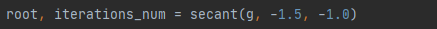
\includegraphics[scale=1]{exercise_1_secant_call_first_root.png}    
        \caption{ Παράδειγμα κλήσης της συνάρτησης \textit{\textlatin{\textbf{secant}}} με αρχικά σημεία \textbf{\textlatin{$x_{0}$ = -1.5}} 
                    και \textbf{\textlatin{$x_{1}$ = -1.0}} .}
    \end{center}
\end{figure}


Μετά την κλήση της συνάρτησης \textit{\textlatin{\textbf{secant}}} τα αποτελέσματα είναι τα εξής:
\vspace{5px}
\begin{figure}[hp]
    \centering
    \captionsetup{justification=centering}
    \begin{center}
    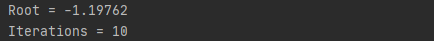
\includegraphics[scale=1]{exercise_1_secant_result_first_root.png}    
    \caption{ Αποτελέσματα κλήσης της συνάρτησης \textit{\textlatin{\textbf{secant}}} \\ με αρχικά σημεία \textbf{\textlatin{$x_{0}$ = -1.5}} 
                και \textbf{\textlatin{$x_{1}$ = -1.0}} . }
    \end{center}
\end{figure}

Όπου παρατηρούμε ότι η ρίζα της \textlatin{\textbf{f(x)}} στο διάστημα \textlatin{\textbf{[-1.5,-1.0]}} με ακρίβεια 5 δεκαδικών ψηφίων 
είναι η \textbf{-1.1976} καθώς και ότι η μέθοδος της τέμνουσας χρειάστηκε \textbf{10} επαναλήψεις για να επιτύχει την 
επιθυμητή ακρίβεια. Στην συνέχεια για την επόμενη ρίζα της \textlatin{\textbf{f(x)}} επιλέγουμε το διάστημα \textlatin{\textbf{[1.3,1.9]}} και
καλούμε την συνάρτηση \textit{\textlatin{\textbf{secant}}} με ορίσματα την συνάρτηση \textlatin{\textbf{f(x)}}, και τα δύο αρχικά σημεία 
\textlatin{\textbf{$x_{0}$= 1.3}} και \textlatin{\textbf{$x_{1}$= 1.9}}.
\vspace{5px}
\begin{figure}[h!]
    \centering
    \captionsetup{justification=centering}
    \begin{center}
        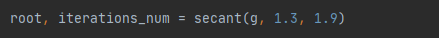
\includegraphics[scale=1]{exercise_1_secant_call_third_root.png}    
        \caption{ Παράδειγμα κλήσης της συνάρτησης \textit{\textlatin{\textbf{secant}}} με αρχικά σημεία \textbf{\textlatin{$x_{0}$ = 1.3}} 
                    και \textbf{\textlatin{$x_{1}$ = 1.9}} .}
    \end{center}
\end{figure}


Μετά την κλήση τα αποτελέσματα είναι τα εξής:
\vspace{5px}
\begin{figure}[h!]
    \centering
    \captionsetup{justification=centering}
    \begin{center}
    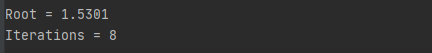
\includegraphics[scale=1]{exercise_1_secant_result_third_root.png}    
    \caption{ Αποτελέσματα κλήσης της συνάρτησης \textit{\textlatin{\textbf{secant}}} \\ με αρχικά σημεία \textbf{\textlatin{$x_{0}$ = 1.3}} 
                και \textbf{\textlatin{$x_{1}$ = 1.9}} . }
    \end{center}
\end{figure}

Όπου παρατηρούμε ότι η ρίζα της \textlatin{\textbf{f(x)}} στο διάστημα \textlatin{\textbf{[1.3,1.9]}} με ακρίβεια 5 δεκαδικών ψηφίων 
είναι η \textbf{1.5301} καθώς και ότι η μέθοδος της τέμνουσας χρειάστηκε \textbf{8} επαναλήψεις για να επιτύχει την 
επιθυμητή ακρίβεια. Τέλος, με την μέθοδο της τέμνουσας αντιμετωπίζουμε το ίδιο πρόβλημα που αντιμετωπίζουν και οι δύο προαναφερόμενες μέθοδοι
για την ρίζα \textbf{\textlatin{x = 0}}. Αν προσπαθήσουμε να καλέσουμε την συνάρτηση \textit{\textlatin{\textbf{secant}}} με αρχικά 
σημεία κάποια σημεία στα οποία δεν τηρούνται όλες οι προϋποθέσεις τα αποτελέσματα είναι μη προβλέψιμα και είτε μπορεί να έχουμε σύγκλιση σε 
λάθος αποτέλεσμα είτε σύγκλιση χωρίς την επιθυμητή ακρίβεια.
\vspace{10mm}
\begin{figure}[h!]
    \centering
    \captionsetup{justification=centering}
    \begin{center}
        \begin{tabular}{ |c|c|c|c| }       
            \hline
            \textbf{\textlatin{$x_{0}$}} & \textlatin{$x_{1}$} & Αποτέλεσμα κλήσης συνάρτησης \textit{\textlatin{\textbf{secant}}} & Αριθμός Επαναλήψεων \\
            \hline
            -0.25 & 0.25 & -0.00002 & 44 \\
            -0.5 & 0.5 & 0.00008 & 46 \\ [1ex]
            \hline
        \end{tabular}
        \caption{ Αποτέλεσματα κλήσεων της συνάρτησης \textit{\textlatin{\textbf{secant}}} χωρίς να τηρούνται όλες οι προϋποθέσεις}
    \end{center}
\end{figure}

Όπως παρατηρούμε και στο σχήμα 21, καμία κλήση δεν βρίσκει την ρίζα της \textlatin{\textbf{f(x)}} με την επιθυμητή ακρίβεια. Η συνάρτηση 
\textit{\textlatin{\textbf{secant}}} που έχει υλοποιηθεί στο αρχείο \textit{\textlatin{\textbf{secant.py}}} έχει τροποποιηθεί έτσι
ώστε να ελέγχει αν κάποιο από τα αρχικά σημεία \textbf{\textlatin{$x_{0}$,$x_{1}$}} αποτελεί ρίζα της \textlatin{\textbf{f(x)}}. Έτσι, αν τώρα
καλέσουμε την συνάρτηση \textit{\textlatin{\textbf{secant}}} με αρχικά σημεία τα \textlatin{\textbf{$x_{0}$= 0}} και 
\textlatin{\textbf{$x_{1}$= 1.5}} παίρνουμε τα εξής αποτελέσματα:
\vspace{5px}
\begin{figure}[h!]
    \centering
    \captionsetup{justification=centering}
    \begin{center}
    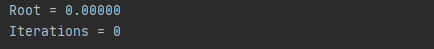
\includegraphics[scale=1]{exercise_1_secant_results_modified_second_root.png}    
    \caption{ Αποτελέσματα κλήσης της τροποποιήμενης συνάρτησης \textit{\textlatin{\textbf{secant}}} \\ με αρχικά σημεία 
                \textbf{\textlatin{$x_{0}$ = 0}} και \textbf{\textlatin{$x_{1}$ = 1.5}} . }
    \end{center}
\end{figure}

Όπου το \textbf{\textlatin{$x_{0}$ = 0}} αποτελεί ρίζα της \textlatin{\textbf{f(x)}}. Τέλος, παρόμοια με την μέθοδο της διχοτόμησης αν και τα 
δύο αρχικά σημεία \textbf{\textlatin{$x_{0}$,$x_{1}$}} αποτελούν ρίζες επιστρέφεται η τιμή του \textbf{\textlatin{$x_{0}$}}.
\newpage
\end{document}